\documentclass{article}
\usepackage{amsmath, amsthm, amssymb, amsfonts}
\usepackage{thmtools}
\usepackage{graphicx}
\usepackage{setspace}
\usepackage{cancel}
\usepackage{geometry}
\usepackage{float}
\usepackage{hyperref}
\usepackage[utf8]{inputenc}
\usepackage[english]{babel}
\usepackage{framed}
\usepackage[dvipsnames]{xcolor}
\usepackage{tcolorbox}
\usepackage{amsmath}
\usepackage{array}
\usepackage{tikz} 
\usepackage{multirow}
\usepackage{tcolorbox}
\usepackage{xcolor}
\usepackage{tikz-cd}
\usepackage{xcolor}
\usepackage{wasysym}

% Define a new color for the example box



\colorlet{LightGray}{White!90!Periwinkle}
\colorlet{LightOrange}{Orange!15}
\colorlet{LightGreen}{Green!15}

\newcommand{\HRule}[1]{\rule{\linewidth}{#1}}

\colorlet{LightGray}{black!10}
\colorlet{LightOrange}{orange!15}
\colorlet{LightGreen}{green!15}
\colorlet{LightBlue}{blue!15}
\colorlet{LightCyan}{cyan!15}



\declaretheoremstyle[name=Theorem,]{thmsty}
\declaretheorem[style=thmsty,numberwithin=section]{theorem}
\usepackage{tcolorbox} % Add missing package
\tcolorboxenvironment{theorem}{colback=LightGray}

\declaretheoremstyle[name=Definition,]{thmsty}
\declaretheorem[style=thmsty,numberwithin=section]{definition}
\tcolorboxenvironment{definition}{colback=LightBlue}

\declaretheoremstyle[name=Proposition,]{prosty}
\declaretheorem[style=prosty,numberlike=theorem]{proposition}
\tcolorboxenvironment{proposition}{colback=LightOrange}


\declaretheoremstyle[name=Example,]{prosty}
\declaretheorem[style=prosty,numberlike=theorem]{example}
\tcolorboxenvironment{example}{colback=LightOrange}

\declaretheoremstyle[name=Axiom,]{prcpsty}
\declaretheorem[style=prcpsty,numberlike=theorem]{axiom}
\tcolorboxenvironment{axiom}{colback=LightGreen}

\declaretheoremstyle[name=Lemma,]{prcpsty}
\declaretheorem[style=prcpsty,numberlike=theorem]{lemma}
\tcolorboxenvironment{lemma}{colback=LightCyan}





\setstretch{1.2}
\geometry{
    textheight=9in,
    textwidth=5.5in,
    top=1in,
    headheight=12pt,
    headsep=25pt,
    footskip=30pt
}

% ------------------------------------------------------------------------------

\begin{document}

% ------------------------------------------------------------------------------
% Cover Page and ToC
% ------------------------------------------------------------------------------

\title{ \normalsize \textsc{}
		\\ [2.0cm]
		\HRule{1.5pt} \\
		\LARGE \textbf{\uppercase{Lecture 7}}
		\HRule{2.0pt} \\ [0.6cm] \LARGE{}
		}

\date{\today}
\author{\textbf{Author} \\ 
		Tom Jeong
        }

\maketitle

\tableofcontents
\newpage

% ------------------------------------------------------------------------------
\section{continuing from last lecture}

\begin{center}
    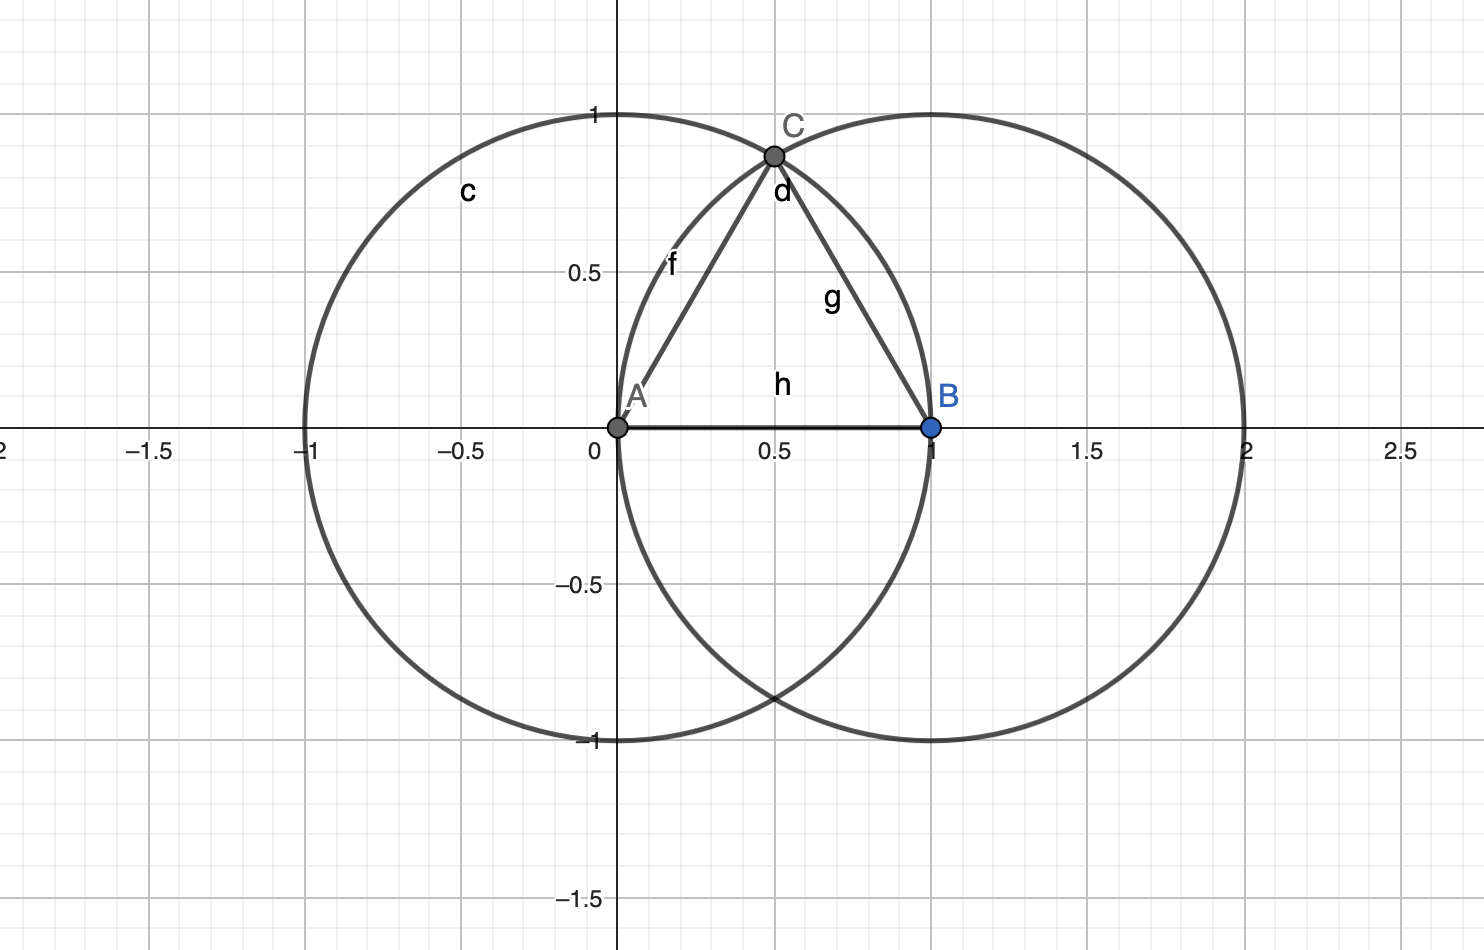
\includegraphics[width=0.5\textwidth]{triangle.png}
\end{center}
a field generated by 0, 1 is $\mathbb{Q}.$ with this equilateral trinalge we generated $\mathbb{Q}(\sqrt{3})$ \\ 
\subsection{intersecting lines }
\begin{align*}
    &\alpha_1 x + \beta_1 y = \gamma_1 \\
    &\alpha_2 x + \beta_2 y = \gamma_2 \\ 
    &\alpha_i, \beta_i, \gamma_i \in K \\ 
    &x, y \in K\\ 
\end{align*}
\subsection{intersecting line with circle }
\begin{align*}
    &\alpha x + \beta y = \gamma \\
    &(x- c_1)^2 + (y-c_2)^2 = r^2 \\ 
    &\text{quadratic in x}
\end{align*}
We may need to add square roots to the field. The degree of extension = 1 or 2. This is because the degree of the extension is the degree of the minimal polynomial. \\ 
Degree $[K : \mathbb{Q}]$ either stays the same or doubles. \\
$[K_{i+1}: \mathbb{Q}] = [K_{i+1} : K_i] \cdot [K_i : \mathbb{Q}]$ \\

\subsection{Intersecting two cricles }
\begin{align*}
    &(x-c_1)^2 + (y-c_2)^2 = r_1^2 \\
    &(x-d_1)^2 + (y-d_2)^2 = r_2^2 \\
    &c_i, d_i, r_i \in K_s
\end{align*}
Solving this system of equations will give us the intersection points. \\
\begin{align*}
    &x^2 - 2c_1x + c_1^2 + y^2 - 2c_2y + c_2^2 = r_1^2 \\
    &x^2 - 2d_1x + d_1^2 + y^2 - 2d_2y + d_2^2 = r_2^2 \\
    &(x-c_1)^2 + (y-c_2)^2 = r_1^2 \\
    &\text{linear equation x of y} \\ 
    &\rightarrow K_o = \mathbb{Q} \\ 
    &[K_s:\mathbb{Q}] = 2^j \quad j \in \mathbb{Z}, j \geq 0
\end{align*}
We must construct $\sqrt[3]{2}$ Using Eisenstein criteria $[\mathbb{Q}(\sqrt[3]{2}) : \mathbb{Q}] = 3$ This is not possible because: 

$$[K_s:\mathbb{Q}] ( = 2^j)= [K_s:\mathbb{Q}(\sqrt[3]{2})] \cdot [\mathbb{Q}(\sqrt[3]{2}):\mathbb{Q}] (=3)$$ 
\section{Trisecting an angle}

\begin{align*}
    &\cos(3\theta) = 4\cos^3(\theta) - 3\cos(\theta) \\ 
    &3\theta \text{is described by a cubic equation} \\
    &3\theta = \frac{\pi}{3} = 60^{\circ} \\
    &\cos(\frac{\pi}{3}) = \frac{1}{2} \\ 
    &\cos(\frac{\pi}{9}) = x \\ 
    &4x^3 - 3x - \frac{1}{2} = 0 \quad \text{if this is reducible we are done} \\ 
    &\text{if yes, then} \quad [\mathbb{Q}(\cos(\frac{\pi}{3})): \mathbb{Q}] = 3\\
    &8x^3 - 6x - 1 = u^3 -3u -1 \\ 
    &\text{where } x = \frac{u}{2} \quad u = 2x \\ 
    &u^3 - 3u - 1 = (au + b)(cu^2 + du + e) \\
    & ac 1 , be = 1 \quad a,b,c,d,e \in \mathbb{Z} \\ 
    &a,c = \pm 1, \quad b,e = \pm 1 \\
    &\rightarrow u = \pm 1 \text{ is a root} \quad  \text{ Gauss' lemma} \\ 
    &\text{but this is not the case}
\end{align*}
\section{Splitting Fields}
$K_, f(x) \in K(x)$
$L$ is a splitting field of $f(x)$ if \begin{enumerate}
    \item $f(x)$ splits into linear factors as polynomial in $L(x)$
    \item $f(x)$ doesn't split into linear factors over any subfield of $L$
\end{enumerate}
We want to show that a splitting field exists and they are unique. 

\begin{lemma}[Existence of Spltting fields] \leavevmode \\ 
    $f(x), K$.. $f = q_1 \hdots q_s$ where $q_i$ is irreducible in $K(x)$ \\
    $K_1 = K(t) / \langle q_1, (t) \rangle$ \\ 
    $t+ \langle q_1(t) \rangle$ is a root of $q_1$ in $K_1$ \\
    factor $f$ as a polynomial in $K_1(x)$. It will have a linear factor \\
    $f = r_1 \hdots r_m$ if $\partial r_i > 1$ \\
    $K_2 = K_1 / \langle r_i(x) \rangle$ \\
    AFter at most n steps we terminate. 
    \\ 
    Built Field $M$ such that $f(x)$ factors into leinear factors in $M(x)$ 
    $\leftrightarrows$ All roots of $f(x)$ lies in $M$ \\ 
    $\alpha_1, \dots \alpha_n$ roots of $f(x)$ in $M$ \\ 
    $L = K(\alpha_1, \dots \alpha_n) \leq M$ \\ 
    $L-$ splitting field of $f(x)$ \\ 
    $[L: K] \leqq n!$ where $n \partial f$ \\ 
    $K{(\alpha_1) : K} \leq n $\\ 
    $K{(\alpha_1, \alpha_2) : K(\alpha_1)} \leq n-1$ \\

\end{lemma}

$f(x) = x^3 - 1$ \\ L splitting fiekd $f(x)$ over $\mathbb{Q}$ 
\\ 
$L = \mathbb{Q}(\sqrt[3]{2}, w\sqrt[3]{2}, w^2\sqrt[3]{2})$ \\
$[\mathbb{Q}(\sqrt[3]{2}): \mathbb{Q}] = 3$ \\
$[\mathbb{Q}(w): \mathbb{Q}] = 2$ \\  
$[L : \mathbb{Q}] = 6$
\end{document}
